%%%%%%%%%%%%%%%%%%%%%%%%%%%%%%%%%%%%%%%%%%%%%%%%%%%%%%%%%%%%%%%%%%%%%%%%%%%%
% Formato en Látex para la generación de material de estudio en la ESPE - DECE 
% Documento generado en base a los formatos ejemplo otorgados por el Ing. Wilson Cerón
% Por:
% Dillan Aldás
% Andres Jimenez
% 
% Last Update: 2020.04.25 
%%%%%%%%%%%%%%%%%%%%%%%%%%%%%%%%%%%%%%%%%%%%%%%%%%%%%%%%%%%%%%%%%%%%%%%%
\documentclass[a4paper, 11pt]{article}
%Paquetes%%%%%%%%%%%%%%%%%%%%%%%%%%%%%%%%%%%%%%%%%%%%%%%%%%%%%%%%%%%%%%%%%%%
\usepackage[utf8]{inputenc}
\usepackage[T1]{fontenc}
\usepackage[spanish]{babel}
\usepackage{everypage}
\usepackage{graphicx}
\usepackage{lipsum}
\usepackage{tikz}
\usepackage{color}
\usepackage[left=3cm, right=2.75cm, top=4.5cm, bottom=4cm]{geometry}
\usepackage{fancyhdr}
\pagestyle{empty}
\usepackage{tikzpagenodes}
\usetikzlibrary{calc}
\usepackage{hyperref}
\usepackage{lipsum}
\usepackage[user,abspage]{zref}
\usepackage{siunitx}
\usepackage[square,numbers]{natbib}
\usepackage[maxbibnames=99, sorting=none, backend=bibtex]{biblatex}
\addbibresource{referencias.bib}
\usepackage{graphicx} 
\usepackage{spanish}
\usepackage{gensymb}
\usepackage{mathptmx}
\usepackage{amsmath}
\usepackage{calc}
\usepackage{latexsym}
\usepackage{amssymb}
%%Comandos y comandos nuevos %%%%%%%%%%%%%%%%%%%%%%%%%%%%%%%%%%%%%%%%%%%%%
%\newcommand{\slink}[2]{\hyperref[#1]{\underline{\smash{#2}}}} 
\renewcommand{\baselinestretch}{1.35} 

%% colores de los hyperlinks - 
% (en Adobe Acrobat los links Sí salen subrayados, en este visor de pdf solo salen azules) 
\hypersetup{%
colorlinks=true, linkcolor=blue, urlcolor=blue,linkbordercolor=blue, citecolor=blue, urlbordercolor=blue, pdfborderstyle={/S/U/W 1}
}
\makeatletter
\Hy@AtBeginDocument{%
  \def\@pdfborder{0 0 1}% Overrides border definition set with colorlinks=true
  \def\@pdfborderstyle{/S/U/W 1}% Overrides border style set with colorlinks=true
                                % Hyperlink border style will be underline of width 1pt
}
\makeatother
%colores%%%%%%%%%%%%%%%%%%%%%%%%%%%%%%%%%%%%%%%%%%%%%%
\definecolor{rojo_oscuro}{rgb}{.85,.45,.45} 
\definecolor{verde_oscuro}{rgb}{0,.5,.2} 
% Formato de todo el documento %%%%%%%%%%%%%%%%%%%%%
\AddEverypageHook{%
\tikz[remember picture,overlay]{%
% Páginas mayores a 2
  \ifnum\value{page}>1%
  % \ifnum\makeatletter\zref@extract{#1}{abspage}\makeatother>1%
  % \ifnum\value{\zref{abspage}}>1%
  % \ifnum\value{page}>1%
    \filldraw[fill=rojo_oscuro, thick,  draw=verde_oscuro] (1,-1.6) rectangle (16,-1.3);
    \filldraw[fill=rojo_oscuro, thick, draw=verde_oscuro] (1,-1.6-22.8) rectangle (16,-1.3-22.8);
        \node[anchor=east] at (16,-25) {\textcolor{black}{{\footnotesize DECE - ESPE}}};
        \node[anchor=west] at (1,-25) {\textcolor{black}{{\footnotesize \thepage}}};
  %logo DECE
        \node at (1.8,0) {\includegraphics[width=2.5cm]{DEEE_LOGO.png}};
%Pagina 1: Carátula%%%%%%%%%%%%%%%%%%%%%%%%%%%%%%%%%%%%%%%%%%%
  \else
    % Márgenes
    \filldraw[fill=rojo_oscuro, thick, draw=verde_oscuro] (-0.3,0) rectangle (0.3,-26); %izquierdo
    \filldraw[fill=rojo_oscuro, thick,  draw=verde_oscuro] (1,-1.6) rectangle (16,-1.3); %arriba
    \filldraw[fill=rojo_oscuro, thick, draw=verde_oscuro] (1,-1.6-21.8) rectangle (16,-1.3-21.8); %abajo
    % Texto de carátula
    \node[anchor=east] at (16,-24) {\textcolor{black}{{\Large Laboratorio de Circuitos eléctricos}}}; 
    \node[anchor=east] at (16,-25) {\textcolor{black}{{\small Procedimiento}}};
    \node[anchor=east] at (16,-25.8) {\textcolor{black}{{\footnotesize 2021}}};
    \node[anchor=east] at (16,-21) {\textcolor{black}{{\Huge Laboratorio 4}}};
    \node[anchor=east] at (16,-22) {\textcolor{black}{{\LARGE Fasores}}};
    %Logos
    \node at (4.2,0.) {\includegraphics[width=6cm]{ESPE_LOGO.png}};
    \node at (14,0.) {\includegraphics[width=2.5cm]{DEEE_LOGO.png}};
 \fi}
 }
%
%
%
%
% \pagenumbering{roman}
%%%%%%%%%%%%%%%%%%%%%%%%%%%%%%%%%%%%%%%%%%%%%%%%%%%%%%%%%%%%%%%%%%%%%%%%%%%%%%%%%%%%%%%%%%%%%%%%%%%%%%%%%%%%%%%%%%%%%%%%%%%%%%%%
\begin{document}
\zlabel{iniciodedocumento}
\textbf{}
\newpage

\begin{flushright}
\textbf{\Huge Contenido}
\end{flushright}

\renewcommand*\contentsname{}
{% color de hyperlinks negro para el índice
\hypersetup{linkcolor=black, urlcolor=black,linkbordercolor=black, urlbordercolor=black, pdfborderstyle={/S/U/W 0.5}}
\tableofcontents
}



\newpage
%\pagenumbering{arabic} % empieza la numeración de página

\section{Procedimiento}

8.5.1 Transforme a su forma polar:

a) 2+3j=

\begin{equation*}
r=\sqrt{2^{2}+3^{2}}=\sqrt{3}=3.60
\end{equation*}
\begin{equation*}
\theta=tan^{-1}(\frac{3}{2})=56.30
\end{equation*}
\begin{equation*}
2+3j=3.60\angle56.30
\end{equation*}

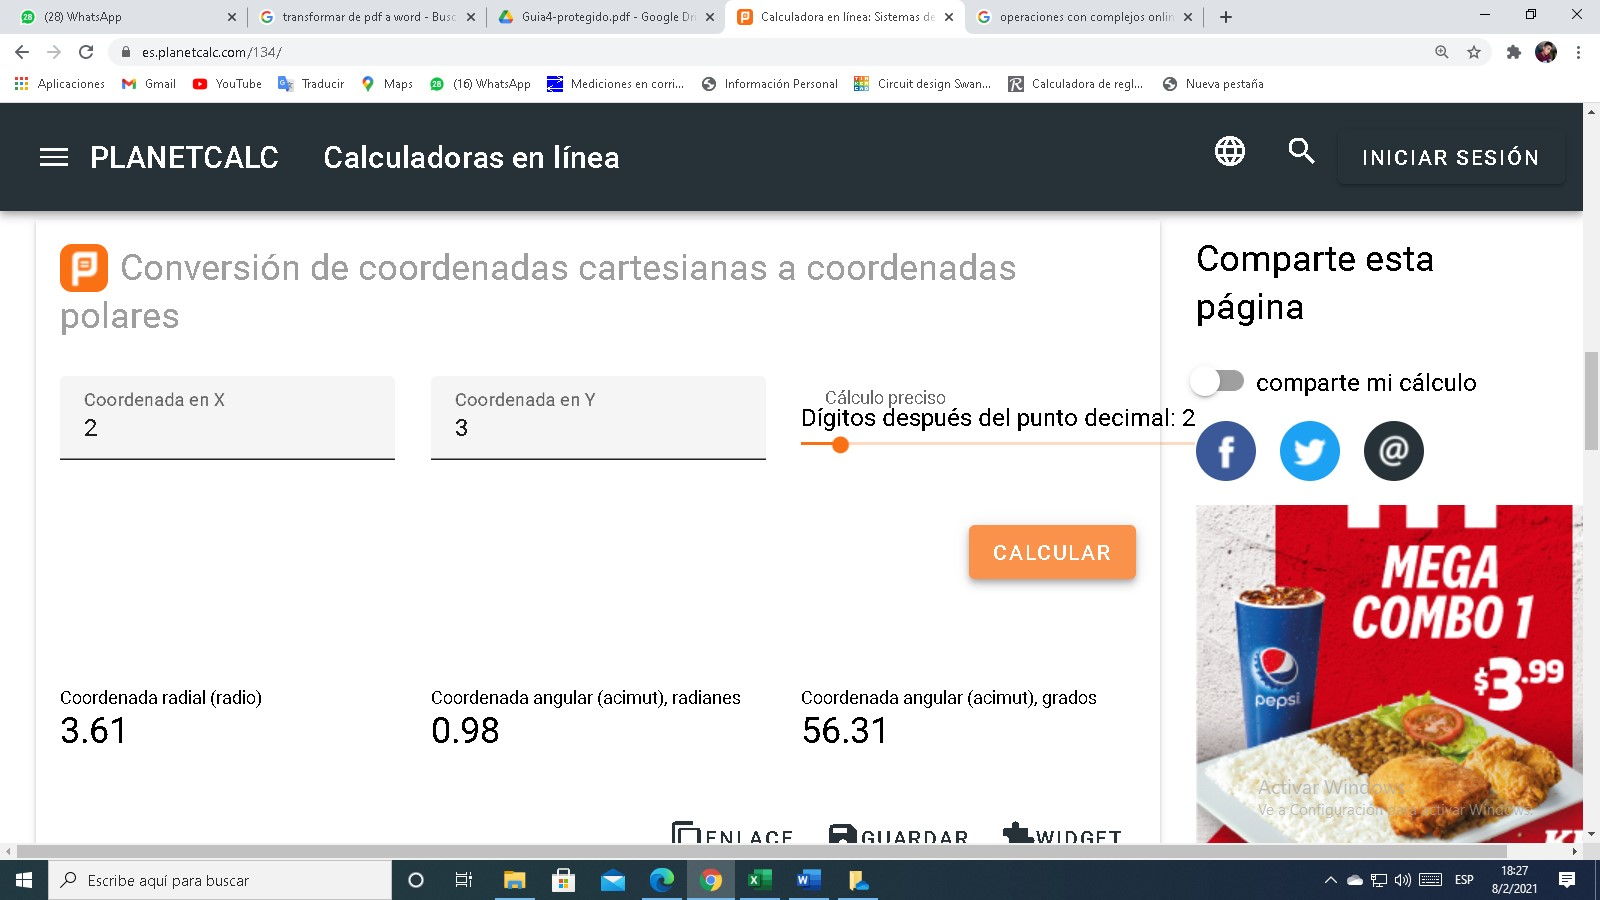
\includegraphics[scale=0.345]{Ejer_8-5-1_lit_a.jpg}

b) -8+6.2j=

\begin{equation*}
r=\sqrt{8^{2}+6.2^{2}}=10.12
\end{equation*}
\begin{equation*}
\theta=tan^{-1}(\frac{6.2}{-8}+180)=-142.23
\end{equation*}
\begin{equation*}
-8+6.2j=10.12\angle142.23
\end{equation*}

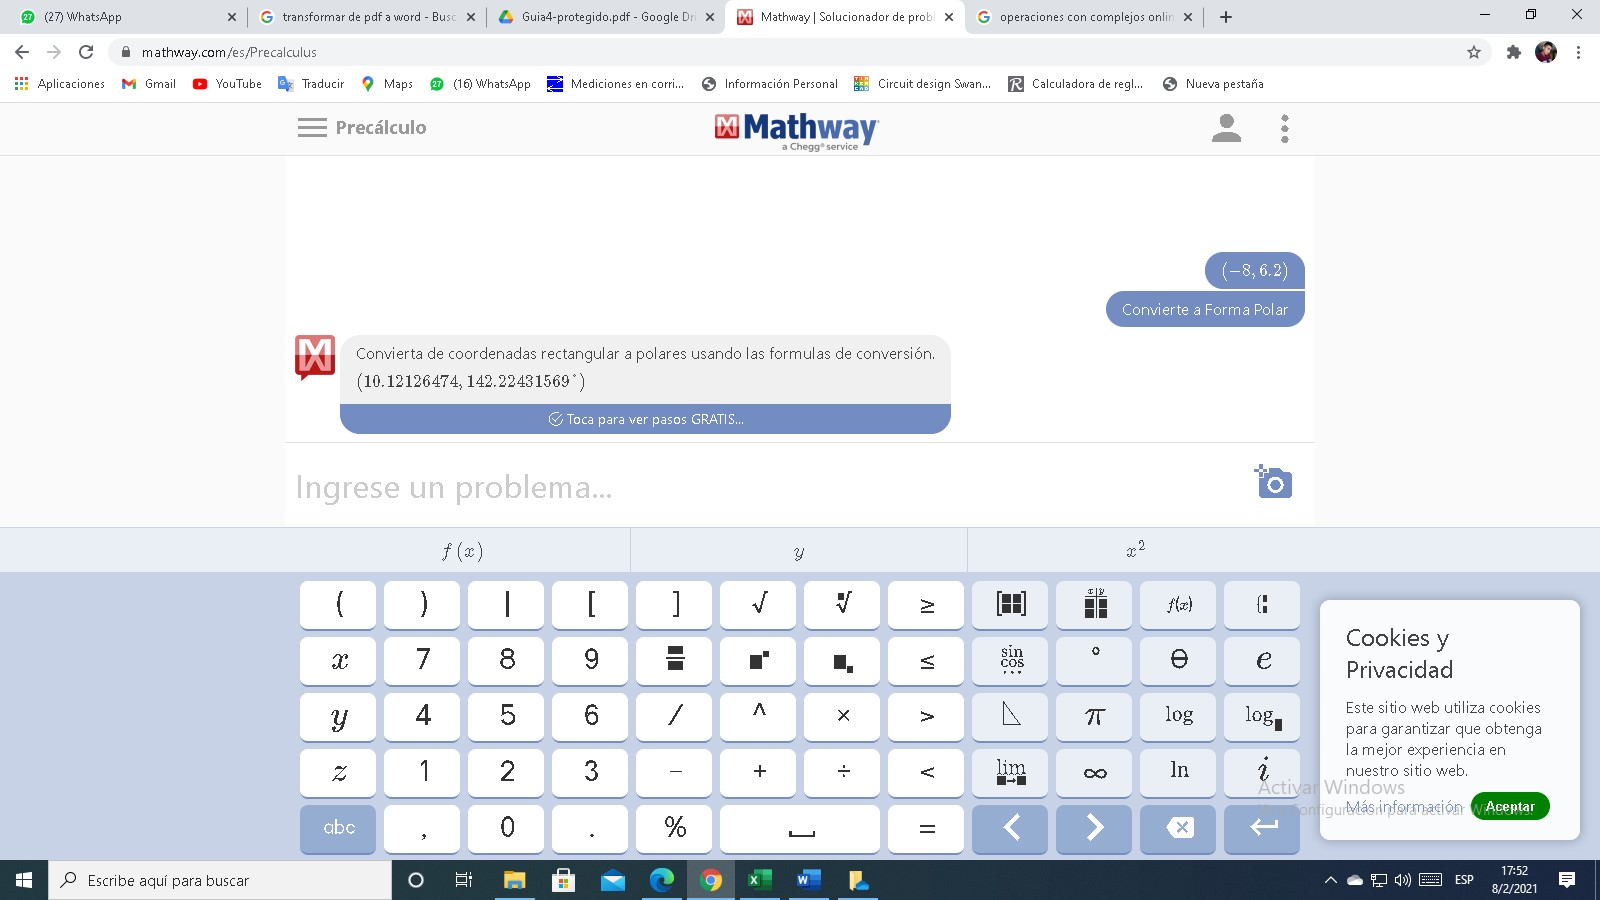
\includegraphics[scale=0.345]{Ejer_8-5-1_lit_b.jpg}

c) 4.3-2.8j=

\begin{equation*}
r=\sqrt{4.3^{2}+2.8^{2}}=5.13
\end{equation*}
\begin{equation*}
\theta=tan^{-1}(\frac{-2.8}{4.3})=-33.07
\end{equation*}
\begin{equation*}
4.3-2.8j=5.13\angle-33.07
\end{equation*}

\includegraphics[scale=0.345]{Ejer_8-5-1_lit_c.jpg}

d) -6-3.2j=

\begin{equation*}
r=\sqrt{6^{2}+3.2^{2}}=6.8
\end{equation*}
\begin{equation*}
\theta=tan^{-1}(\frac{-3.2}{-6})-180=-151.93
\end{equation*}
\begin{equation*}
-6-3.2j=6.8\angle-151.93
\end{equation*}

\includegraphics[scale=0.345]{Ejer_8-5-1_lit_d.jpg}

8.5.2 Transforme a su forma rectangular:

a) $36\angle-10$=

\begin{equation*}
x=36cos(-10)=35.45
\end{equation*}
\begin{equation*}
y=36sen(-10)=-6.25j
\end{equation*}
\begin{equation*}
36\angle-10=35.45-6.25j
\end{equation*}

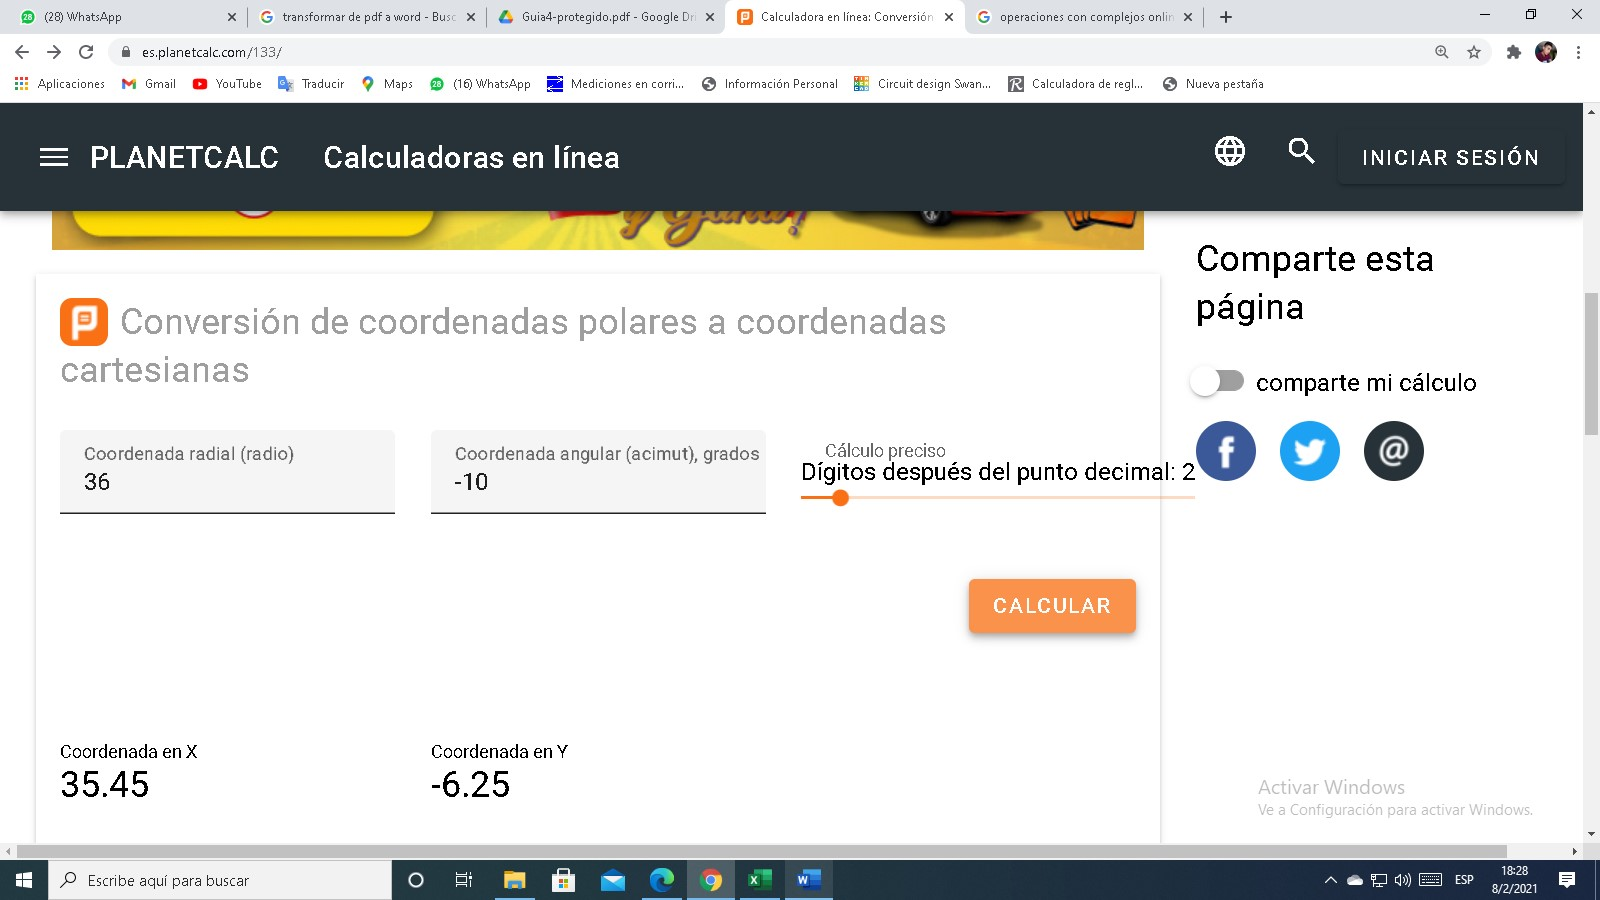
\includegraphics[scale=0.345]{Ejer_8-5-2_lit_a.jpg}

b) $28.7\angle135$=

\begin{equation*}
x=28.7cos(135)=-20.29
\end{equation*}
\begin{equation*}
y=28.7sen(135)=20.29j
\end{equation*}
\begin{equation*}
28.7\angle135=-20.29+20.29j
\end{equation*}

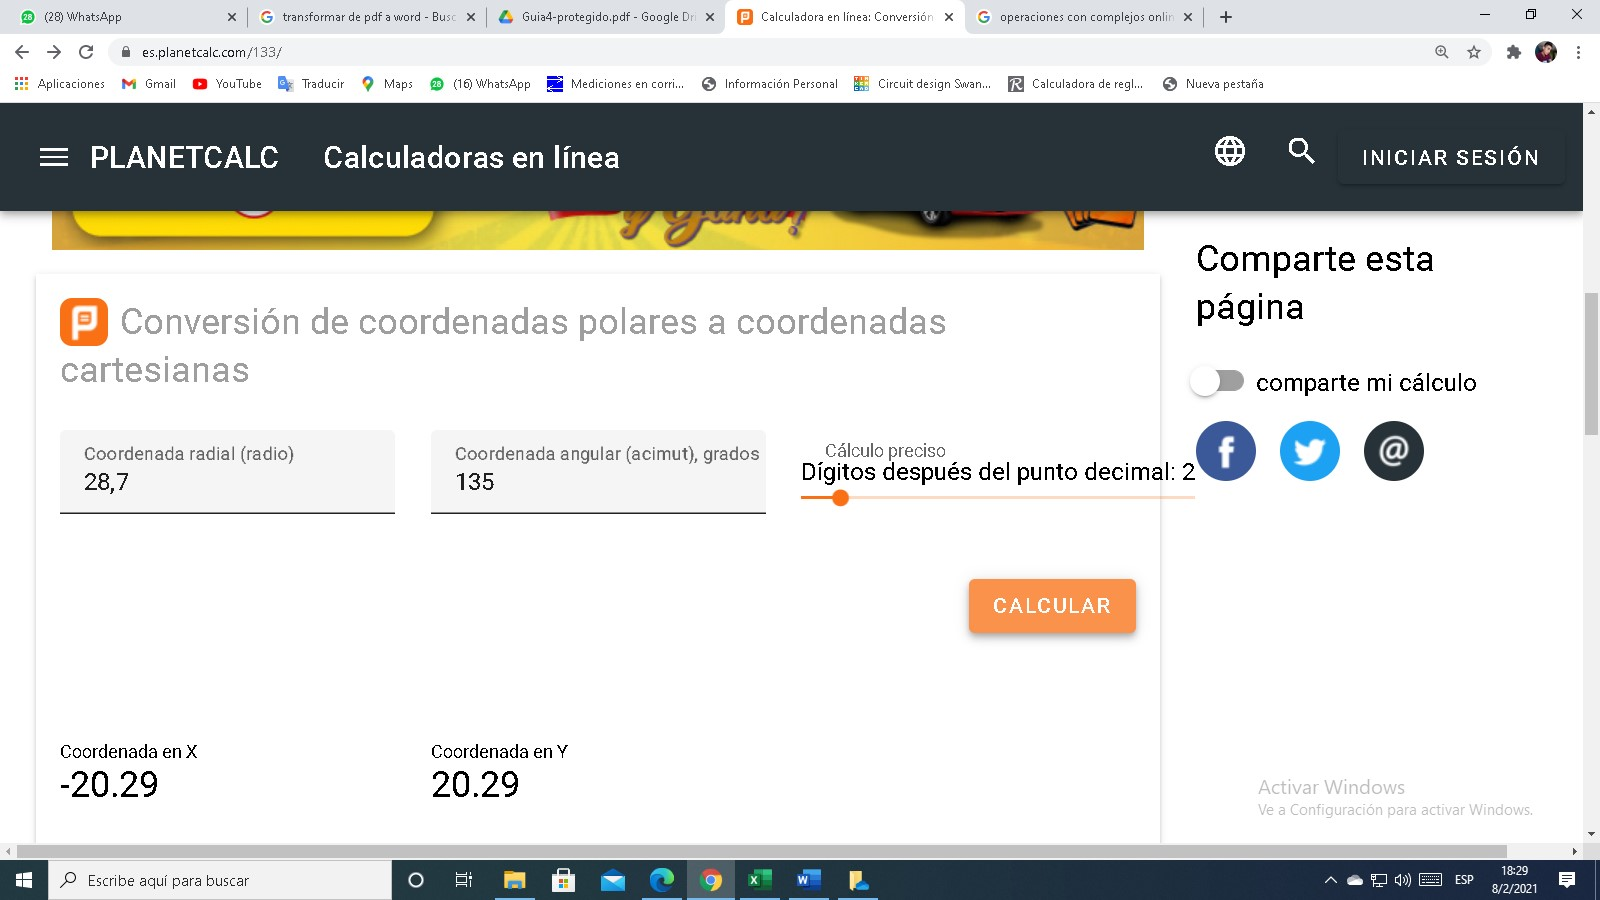
\includegraphics[scale=0.345]{Ejer_8-5-2_lit_b.jpg}

c) $11.2\angle28$=

\begin{equation*}
x=11.2cos(28)=9.88
\end{equation*}
\begin{equation*}
y=11.2sen(28)=5.25j
\end{equation*}
\begin{equation*}
11.2\angle28=9.88+5.25j
\end{equation*}

\includegraphics[scale=0.345]{Ejer_8-5-2_lit_c.jpg}

d) $45\angle-117.9$=

\begin{equation*}
x=45cos(-117.9)=-21.02
\end{equation*}
\begin{equation*}
y=45sen(-117.9)=-39.76j
\end{equation*}
\begin{equation*}
45\angle-117.9=-21.05-39.76j
\end{equation*}

\includegraphics[scale=0.345]{Ejer_8-5-2_lit_d.jpg}

8.5.2 Realice las siguientes operaciones paso a paso, y represente el resultado tanto en su forma rectangular como en su forma polar.

a) $\frac{10+3j}{2j}-(7+2j)(3\angle-115)$

\begin{equation*}
\frac{10.44\angle16.69}{2\angle90}-(7.28\angle15.94)(3\angle-115)
\end{equation*}
\begin{equation*}
(5.22\angle-73.31)-(21.84\angle-99.06)
\end{equation*}
\begin{equation*}
1.49-5j-(-3.44-21.56j)
\end{equation*}

Forma rectangular= $4.93+16.56j$ 

Forma polar= $17.27\angle73.42$

\includegraphics[scale=0.94]{Ejer_8-5-3_lit_a1.jpg}

\includegraphics[scale=0.94]{Ejer_8-5-3_lit_a2.jpg}

b) $6.8\angle125.3+\frac{4.5\angle-11.5}{7.6-1.2j}$

\begin{equation*}
6.8\angle125.3+\frac{4.5\angle-11.5}{7.69\angle-8.97}
\end{equation*}
\begin{equation*}
6.8\angle125.3+(0.58\angle-2.53)
\end{equation*}
\begin{equation*}
-3.92+5.54j+0.57-0.025j
\end{equation*}

Forma rectangular= $-3.35+5.51j$ 

Forma polar= $6.44\angle121.19$

\includegraphics[scale=0.94]{Ejer_8-5-3_lit_b1.jpg}

\includegraphics[scale=0.94]{Ejer_8-5-3_lit_b2.jpg}

c) $\frac{34+28.5j}{4\angle-20.8}-51.2\angle215$

\begin{equation*}
\frac{44.36\angle39.97}{4\angle-20.8}-(-41.94-29.36j)
\end{equation*}
\begin{equation*}
(11.09\angle60.97)+41.94+29.36j)
\end{equation*}
\begin{equation*}
5.38+9.69j+41.94+29.36j
\end{equation*}

Forma rectangular= $47.32+39.05j$ 

Forma polar= $61.35\angle39.53$

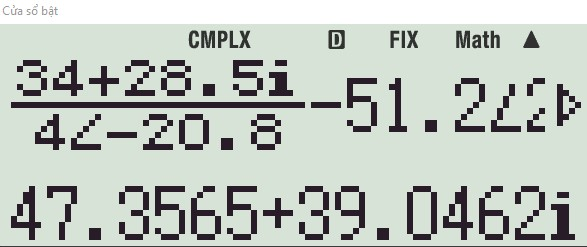
\includegraphics[scale=0.94]{Ejer_8-5-3_lit_c1.jpg}

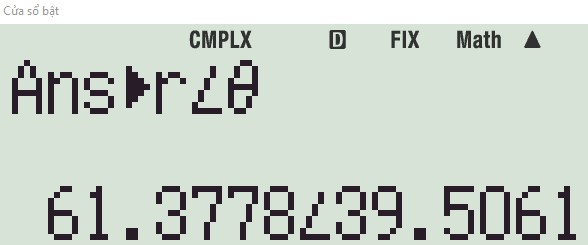
\includegraphics[scale=0.94]{Ejer_8-5-3_lit_c2.jpg}

\end{document}